\documentclass{article}
\usepackage[T1]{fontenc}
\usepackage{lmodern}
\usepackage{graphicx}
\usepackage{amsmath,amssymb}
\usepackage[a4paper,margin=2cm]{geometry}
\usepackage[absolute,overlay]{textpos}
\setlength{\TPHorizModule}{1mm}
\setlength{\TPVertModule}{1mm}
\usepackage[indonesian]{babel}
\usepackage{hyperref}
\setlength{\emergencystretch}{2em}
% unit: Halaman 18

\begin{document}

% === Halaman 18 (llm) ===

\begin{itemize}
    \item Gambar \textit{man-in-the-middle attack} berikut memperlihatkan cara Mallory menyepakati kunci yang sama dengan Alice ($K_1 = g^{am} \pmod{p}$) dan menyepakati kunci yang sama dengan Bob ($K_2 = g^{bm} \pmod{p}$)
    \vspace{40mm}
    \item Ketika Alice mengirim $g^a \pmod{p}$ kepada Bob, Mallory mengintersepsi komunikasi dan menggantikannya dengan $g^m \pmod{p}$ lalu mengirimkannya kepada Bob
    \item Ketika Bob mengirim $g^b \pmod{p}$ kepada Alice, Mallory mengintersepsi komunikasi dan menggantikannya dengan $g^m \pmod{p}$ lalu mengirimkannya kepada Alice.
    \item Alice menghitung $K_1 = g^{am} \pmod{p}$, sama dengan yang dihitung Mallory, $K_1 = g^{am} \pmod{p}$
    \item Bob menghitung $K_2 = g^{bm} \pmod{p}$, sama dengan yang dihitung Mallory, $K_2 = g^{bm} \pmod{p}$
    \item Selanjutnya Mallory mengetahui pesan2 rahasia dari Alice dan dari Bob yang dienkripsi dengan dengan kunci $K_1$ dan $K_2$ tersebut
\end{itemize}

\vspace{10mm}

Sumber gambar: \url{https://textbook.cs161.org/crypto/key-exchange.html}

\hfill Rinaldi M/I4020 Kriptografi

% deskripsi: Diagram serangan man-in-the-middle pada pertukaran kunci Diffie-Hellman yang melibatkan Alice, Mallory, dan Bob.
% bbox normalisasi: [0.5200, 0.2700, 0.9500, 0.8300]
\begin{textblock*}{90.30mm}(109.20mm,80.19mm)
\noindent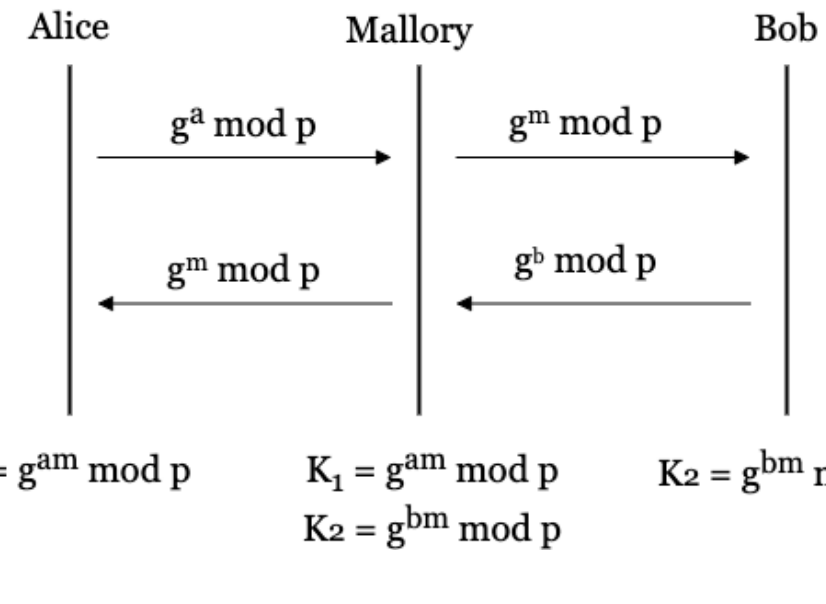
\includegraphics[width=90.30mm,height=166.32mm]{../../images/llm/page_018_img_01.png}%
\end{textblock*}

\end{document}
